\section{Experiments}
\label{sec:experiments}
In this section, we first introduce the experimental setup. We then evaluate our method across different quantization precisions, demonstrating its ability to significantly reduce activation bit requirements compared to existing methods across multiple datasets. Additionally, we conduct comprehensive ablation studies and present visualizations of generated images to assess the effectiveness of MoDiff.

\subsection{Experiment Settings}
\label{subsec:setting}
\textbf{Datasets, Models, and Evaluation.} We majorly evaluate the effectiveness of our MoDiff on the CIFAR-10 (\(32 \times 32\)), LSUN-Bedrooms (\(256 \times 256\)), and LSUN-Church-Outdoor (\(256 \times 256\)) datasets~\citep{krizhevsky2009learning, yu15lsun}. For CIFAR-10, we use DDIM models with 100 denoising steps~\citep{song2020denoising}. For the LSUN datasets, we use Latent Diffusion Models with downsampling factors of 4 and 8, referred to as LDM-4 (Bedrooms) and LDM-8 (Churches), respectively~\citep{rombach2022high}. We use 500 sampling steps for LDM-4 and 200 steps for LDM-8. To demonstrate the generalization capability of MoDiff across datasets and architecture, we also conduct experiments on Stable Diffusion and Transformer-based models~\citep{peebles2023scalable} on MS-COCO~\citep{lin2014microsoft} and ImageNet~\citep{ILSVRC15}, respectively. Additional details and results are provided in Appendix~\ref{appse: stable} and \ref{appsec: DiT}.

We assess generation quality using Inception Score (IS)~\citep{salimans2016improved}, Fr\'echet Inception Distance (FID)~\citep{heusel2017gans}, and Sliced Fr\'echet Inception Distance (sFID)~\citep{salimans2016improved} for CIFAR-10, and FID and sFID for the LSUN, as IS is not a reliable metric for datasets that significantly deviate from ImageNet categories. All metrics are computed based on 50,000 generated images. Additionally, we provide precision and recall measurements~\citep{sajjadi2018assessing} in Appendix~\ref{appsec:measurements}.  

\textbf{Quantization Methods.} We use dynamic channel-wise quantization and Q-Diffusion as the base quantization methods and apply MoDiff to both~\citep{dettmers2022gpt3,li2023q}. We also present results using dynamic tensor-wise quantization in Appendix~\ref{subsec:tensor}. Additionally, we include results with full-precision activation (32 bits), for comparison. For weight quantization, we adopt the MSE reconstruction method, following the Q-Diffusion checkpoints. For activation quantization, dynamic channel-wise quantization determines the scaling factor based on the channel-wise min-max range of the input. Due to its dynamic nature, we directly apply MoDiff to this method. In contrast, Q-Diffusion optimizes the scaling factor by minimizing the MSE reconstruction loss using calibration datasets across different time steps. To apply MoDiff to Q-Diffusion, we calibrate the activation quantizers by inputting the calibration datasets into our MoDiff and learn the scaling factors with the residual. Additional implementation details can be found in Appendix~\ref{appsec:implement}. We also perform few-step generation experiments using MixDQ~\citep{zhao2024mixdq} as the baseline, with results provided in Appendix~\ref{appsec:fewstep}.

For quantization hyperparameters, we select weight bit widths from \(\{4, 8\}\) and activation bit widths from \(\{2, 3, 4, 6, 8\}\). For notation simplicity, we use the format \textbf{``W/A"}, where ``W" represents the weight precision and ``A" represents the activation precision. We refer to Q-Diffusion and dynamic channel-wise quantization as \textbf{LCQ} and \textbf{Q-Diff}, respectively. Our implementations based on them are denoted as \textbf{LCQ+MoDiff} and \textbf{Q-Diff+MoDiff}. We denote full-precision activation models as \textbf{Full Prec. (Act)}.

\begin{remark}
The primary objective of this paper is to demonstrate the effectiveness of our method. We do not report the real acceleration metrics, such as running time. Following existing works~\citep{li2023q,wang2024towards}, we evaluate efficiency by measuring the number of binary operations (Bops) per denoising step for a single image with the help of DeepSpeed~\citep{song2023deepspeed4science}. Implementing acceleration on specialized hardware is beyond the scope of this work, but will be a promising future direction, which is plausible given the increasing hardware support for low-precision formats such as 4-bit integers~\citep{nvidiaint4}.
\end{remark}

\subsection{Main Results on CIFAR10 and LSUN}
\label{subsec:results}
\begin{table}[t!]
\small
\caption{The IS, FID, sFID, and GBOPs for LSUN-Church with LDM-8 under different precisions.}
\resizebox{0.45\textwidth}{!}{
\begin{tabular}{l|c|c|cc}
\toprule
{Methods} & {Bits (W/A)} & GBops & FID $\downarrow$ & sFID $\downarrow$ \\
\midrule
Full Prec. (Act) & 8/32 &{5015} & 4.03 & 10.89 \\
\midrule
Q-Diff & \multirow{4}{*}{8/8} & \multirow{4}{*}{1254} & 4.24 & 10.57 \\
Q-Diff+MoDiff (Ours) & & & \bf 3.85 & 10.82 \\
LCQ & & & 4.02 & 11.53 \\
LCQ+MoDiff (Ours) & & & 3.99 &\bf  10.06 \\
\midrule
Q-Diff & \multirow{4}{*}{8/6} & \multirow{4}{*}{1254} & 55.13 & 30.98 \\
Q-Diff+MoDiff (Ours) & & & 5.43 & 13.41 \\
LCQ & & & 4.50 & 12.90 \\
LCQ+MoDiff (Ours) & && \bf 3.89 & \bf 10.12 \\
\midrule
Q-Diff & \multirow{4}{*}{8/4} & \multirow{4}{*}{1254} & 355.85 & 187.56 \\
Q-Diff+MoDiff (Ours) & & & \bf 3.97 & 11.16 \\
LCQ & & & 198.37 & 161.03 \\
LCQ+MoDiff (Ours) & && 34.02 & \bf 10.59 \\
\midrule
Q-Diff & \multirow{4}{*}{8/3} & \multirow{4}{*}{1254} & 367.51 & 354.59 \\
Q-Diff+MoDiff (Ours) & & & \bf 5.40 & \bf 13.81 \\
LCQ & & & 341.62 & 407.68 \\
LCQ+MoDiff (Ours) && & 12.05 & 35.29 \\
\bottomrule
\end{tabular}
}
\label{tab:church}
\end{table}


We conducted experiments to generate images using quantized diffusion models and measure their quality. The IS, FID, and sFID scores for CIFAR-10, Churches, and Bedrooms are presented in Tables~\ref{tab:cifar10}, \ref{tab:church}, and \ref{tab:bedroom}, respectively. Due to page limitations, we only present results for 8-bit weight quantization on the LSUN datasets here. For results with 4-bit weight quantization, please refer to Appendix~\ref{appsec:otherwp}. We highlight the best performance in bold. Based on these results, we draw the following conclusions.

\textbf{Generation Quality.} Our method preserves high generation quality and significantly outperforms the base quantization approach when using lower activation precision across different quantization methods and datasets. Specifically, with LCQ+MoDiff, activation precision in dynamic quantization can be reduced to 3 bits for CIFAR-10 without sacrificing generation quality. In contrast, the base quantization method experiences a significant performance drop even at 6-bit activation precision. For example, the sFID score of Q-Diff on CIFAR-10 degrades from 4.49 to 13.81. Furthermore, even at 2-bit activation precision, our method maintains an sFID of 8.42 on CIFAR-10.

\textbf{Generality.} Our method is generalizable across different datasets and various quantization methods. For both Q-Diff and LCQ, our approach consistently improves their performance. However, we observe that quantizing activations to extremely low-bit precision becomes increasingly challenging for higher-resolution datasets, even with our method. As shown in Tables~\ref{tab:church} and \ref{tab:bedroom}, the FID and sFID scores increase significantly at 3-bit precision for the Churches dataset and become notably high at 4-bit precision for the Bedrooms dataset. This challenge arises because LDMs are deeper and contain higher-dimensional hidden embeddings, making it more difficult to minimize quantization error.

\textbf{Efficiency.} As shown in Tables~\ref{tab:cifar10}, \ref{tab:church}, and \ref{tab:bedroom}, our method consistently reduces binary operations (Bops) for generation. For a full-precision activation model, one denoising step in CIFAR-10 requires 1636 GBops. In contrast, LCQ+MoDiff completes inference with only 154 GBops without any performance degradation, achieving over $10\times$ computational savings. However, the generation quality (sFID) begins to degrade at 8/6-bit precision, which requires 307 GBops.
\begin{table}[t!]
\small
\centering
\caption{The IS, FID, sFID, and GBOPs for LSUN-Bedrooms with LDM-4 under different precisions. 
}
\resizebox{0.45\textwidth}{!}{
\begin{tabular}{l|c|c|cc}
\toprule
{Methods} & {Bits (W/A) } & GBops & FID $\downarrow$ & sFID $\downarrow$ \\
\midrule
Full Prec. & 8/32 & 25560 & 3.45 & 8.45 \\
\midrule
LCQ & \multirow{2}{*}{8/8} & \multirow{2}{*}{6390}& 3.61 & 8.65 \\
LCQ+MoDiff (Ours) & && \bf 3.57 & \bf 8.44 \\
\midrule
LCQ & \multirow{2}{*}{8/6}&\multirow{2}{*}{4609} & 64.17 & 63.18 \\
LCQ+MoDiff (Ours) & && \bf 3.57 & \bf 6.53 \\
\midrule
LCQ & \multirow{2}{*}{8/4}&\multirow{2}{*}{3195} & 372.30 & 262.11 \\
LCQ+MoDiff (Ours) & && \bf 27.88 & \bf 77.85 \\
\bottomrule
\end{tabular}
}
\vspace{-0.1in}
\label{tab:bedroom}
\end{table}



\subsection{Ablation Study}
\label{subsec:ablation}
In this section, we conduct ablation studies to analyze the effectiveness of MoDiff. First, we evaluate the impact of error-compensation modulation. Next, we demonstrate the compatibility of MoDiff with different samplers. Additionally, we examine how our method balances the trade-off between memory and computational efficiency. Finally, we present visualization results to further illustrate the effectiveness of MoDiff in Appendix~\ref{app:visualize}. {To further demonstrate the generalization of MoDiff, we also include results on few-step diffusion models, as presented in the Appendix~\ref{appsec:fewstep}.}

\begin{table}[t!]
\centering
\small
\caption{FID on CIFAR-10 using the DDIM sampler in the ablation study of error compensation. ``EC'' denotes error compensation and the best performance is \textbf{bolded}.}
\begin{tabular}{c|c|cc}
\toprule
\multirow{2}{*}{\centering {Bits (W/A)}} & \multirow{2}{*}{\centering {LCQ}} & \multicolumn{2}{c}{{LCQ+MoDiff}} \\
& & w/o EC & w/ EC \\
\midrule
8/8 & 4.61 & 4.41 & \textbf{4.40} \\
8/6 & 13.07 & 10.21 & \textbf{4.38} \\
8/4 & 33.97 & 25.42 & \textbf{4.38} \\
\bottomrule
\end{tabular}
\vspace{-0.1in}
\label{tab:error_compensation}
\end{table}

\begin{figure}[h!]
    \centering
    \vspace{-0.1in}
    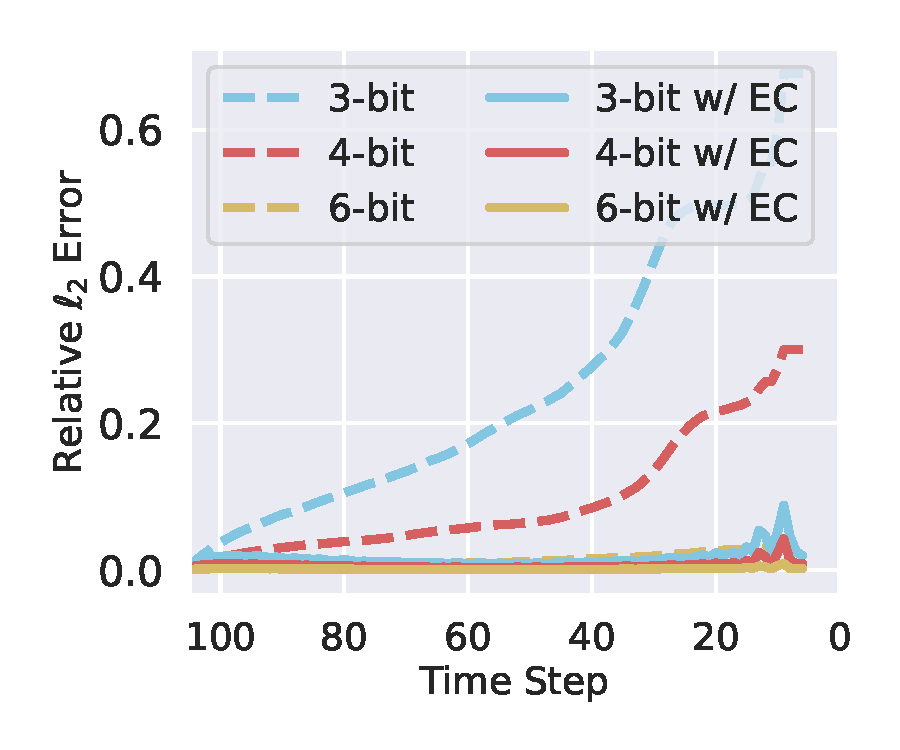
\includegraphics[width=0.7\linewidth]{figures/error_com.pdf}
    \vspace{-0.1in}
    \caption{The relative \(\ell_2\) distance between the features in the standard diffusion model and the quantized model in \textit{middle block}. ``w/ EC" denotes the use of the error-compensation technique.}
    \label{fig:error_comp}
\end{figure}

\textbf{Effects of error compensation} We demonstrate how the error compensation technique mitigates error accumulation by comparing both generation quality and the quantization error, using DDIM on CIFAR-10 with LCQ. FIDs are shown in Table~\ref{tab:error_compensation}. To quantify quantization error, we compute the relative $\ell_2$ distance between the features of \textit{middle block} in the standard diffusion model and the quantized model, both initialized from the same noise. As shown in Figure~\ref{fig:error_comp}, the dashed line represents the relative error without error compensation, while the solid line represents the error with compensation. Without error compensation, error accumulation becomes significant below 6-bit precision. In contrast, with error compensation, the error remains minimal, even at 3-bit precision. In summary, our technique effectively avoids error accumulation in modulated computing.

\textbf{Different Samplers} We demonstrate that MoDiff is compatible with different samplers in diffusion models. While DDIM is used as the sampler in our main experiments, we also evaluate our method with DDPM on LCQ using the LSUN-Bedroom dataset, as shown in Table~\ref{tab:solver}. Our results indicate that MoDiff enhances the generation quality of DDPM, particularly at lower activation bit widths. However, the improvement is less pronounced compared to DDIM. This is because the DDPM sampler introduces random noise at each step, increasing the difference between adjacent features. Consequently, this leads to larger residual magnitudes, which in turn amplify quantization errors. {We provide additional experiments on PLMS~\citep{liu2022pseudo} and DPM solver~\citep{lu2022dpm} in Appendix~\ref{appsec:sampler}.}

\begin{table}[t!]
\small
\centering
\caption{FID and sFID on LSUN-Bedrooms using the DDPM sampler under different quantization precisions with LCQ. The best performance is \textbf{bolded}.}
\resizebox{0.45\textwidth}{!}{
\begin{tabular}{l|c|cc}
\toprule
{Methods} & {Bits (W/A)} & FID $\downarrow$ & sFID $\downarrow$ \\
\midrule
LCQ (DDPM) & \multirow{2}{*}{8/8} & 3.61 & 8.65 \\
LCQ+MoDiff (DDPM) & & \bf 3.39 & \bf 8.02  \\
\midrule
LCQ (DDPM) & \multirow{2}{*}{8/6} & 50.17 & 52.18\\
LCQ+MoDiff (DDPM) & & \bf 12.60 & \bf 13.71  \\
\midrule
LCQ (DDPM) & \multirow{2}{*}{8/4} & 102.16 & 104.18 \\
LCQ+MoDiff (DDPM) & & \bf 34.25 & \bf 30.12  \\
\bottomrule
\end{tabular}}
\vspace{-0.1in}
\label{tab:solver}
\end{table}



\textbf{Memory Consumption.} As discussed in Section~\ref{sec:method}, our method reduces quantization error at the cost of slightly increased memory usage. In Table~\ref{tab:memory}, we demonstrate that MoDiff significantly reduces Bops at lower bit precision while maintaining manageable memory overhead. The results show that the memory overhead is minimal—no more than 4 MB. For more details, we refer to Appendix~\ref{appsec:memory}.

\begin{table}[ht!]
\small
\centering
\vspace{-0.1in}
\caption{The relationship between BOPs and memory usage of our method using DDIM on CIFAR-10 for generating a single image.}
\begin{tabular}{l|ccc|c}
\toprule
{Measurement} & {W8A2} & {W8A4} & {W8A8} & {W8A32} \\
\midrule
sFID & 8.42 & 4.38  & 4.39 & 4.41 \\
GBops & 102 & 205 & 409 & 1636 \\
Memory (Mb) & 35.28 & 36.4 & 38.89 & 35.09 \\
\bottomrule
\end{tabular}
\vspace{-0.1in}
\label{tab:memory}
\end{table}


